
\chapter{\uppercase{Solution}}

\section{Overview}

I propose a new DNS system for Tor hidden services, which I am calling EsgalDNS. \textit{Esgal} is a Sindarin Elvish noun from the works of J.R.R Tolkien, meaning "veil" or "cover that hides".\cite{SindarinDict} EsgalDNS is a distributed DNS system embedded within the Tor network on top of the existing Tor hidden service infrastructure. EsgalDNS shares some design principles with Namecoin and other DNS systems, and its usage is similar to the traditional Clearnet DNS system. At a high level, the system is powered at any given time by a randomly-chosen subset of Tor nodes, whose primary responsibilities are to receive new DNS records from hidden service operators, propagate the records to all parties, and save the records in a main long-term data structure. Other Tor nodes may mirror this data structure, distributing the load and responsibilities to many Tor nodes. The system supports a variety of command and control operations including Query, Create, Modify, Move, Renew, and Delete. 

\section{Components}

\subsection{Cryptographic Primitives}

Our system makes use of cryptographic hash algorithms, digital signatures, proof-of-work, and a pseudorandom number generator. As the cryptographic data within our system must persist for many years to come, we select well-established algorithms that we predict will remain strong against cryptographic analysis in the immediate future.

\begin{itemize}
	\item Hash function - We choose SHA-384 for most applications for its greater resistance to preimage, collision, and pseudo-collision attacks over SHA-256, which is itself significantly stronger than Tor's default hidden service hash algorithm, SHA-1. Like SHA-512, SHA-384 requires 80 rounds but its output is truncated to 48 bytes rather than the full 64, which saves space.
	\item Digital signatures - Our default method is EMSA-PSS, (EMSA4) a probabilistic signature scheme defined by PKCS1 v2.1 and republished in 2003's RFC 3447, using a Tor node's 1024-bit RSA key with the SHA-384 digest to form the signature appendix. For signatures inside our proof-of-work scheme, we rely on $EMSA-PKCS1-v1_5$, (EMSA3) defined by 1998's RFC 2315. In contrast to EMSA-PSS, its deterministic nature prevents hidden service operators from bypassing the proof-of-work and brute-forcing the signature to validate the record.
	\item Proof-of-work - We select scrypt, a password-based key derivation function which is notable for its large memory and CPU requirements during its operation. The scrypt function provides significantly greater resistance to custom hardware attacks and massively parallel computation primarily due to its memory requirements. This limits attackers to the same software implementation and asymptotic cost as legitimate users.\cite{percival2009stronger} We choose scrypt because of these advantages over other key derivation functions such as SHA-256 or PBKDF2.
	\item Pseudorandom number generation - In applications that require pseudorandom numbers from a known seed, we use the Mersenne Twister generator. In all instances the Mersenne Twister is initialized from the output of a hash algorithm, negating the generator's weakness of producing substandard random output from certain types of initial seeds.
\end{itemize}

We use the JSON format to encode records and databases of records. JSON is significantly more compact than XML, but retains readability. Its support of basic primitive types is highly applicable to our needs. Additionally, we consider the JSON format safer than byte-level encoding.

\subsection{Quorum}

As a distributed system, EsgalDNS may have many participants; any machine with sufficient storage and bandwidth capacity --- including those outside the Tor network --- may perform a full synchronization with the EsgalDNS network and obtain a full mirror of all DNS information. Inside the Tor network, these participants are divided into three main categorizes: \textit{quorum} nodes, quorum node \textit{candidates}, and \textit{mirrors}. \textit{Mirrors} are Tor nodes that have performed a full synchronization and hold a complete copy of all DNS data structures. However, they are either not qualified or have opted out of being a quorum node \textit{candidate}. The requirements to become a candidate are described in the next section. Of those that qualify, the \textit{quorum} is chosen as a random subset from the \textit{candidate} list. The \textit{quorum} perform the main duties of the system, namely broadcasting and recording DNS records from hidden service operators. 

Any party at any time may derive the list of \textit{candidate} nodes and the \textit{quorum} from them by the following procedure:

\begin{enumerate}
	\item Obtain a remote or local archived copy of the consensus document, $ cd $, published 00:00 GMT that morning.
	\item Extract the digital signature and verify $ cd $ against $ PK_{authorities} $.
	\item Construct a numerical list, $ ql $ of qualified Tor nodes (defined below) from $ cd $.
	\item Initialize the Mersenne Twister PRNG with SHA-384($ cd $).
	\item Use the seeded PRNG to randomly scramble $ ql $.
	\item Let the first $ M $ nodes, numbered $ 1 .. M $, define the \textit{quorum}.
\end{enumerate}

%\begin{figure}[htbp]
%	\centering
%	\begin{tikzpicture}[->, >=stealth', shorten >=1pt, auto, node distance=2.5cm,
%			thick, main node/.style={circle, fill=blue!20, draw, font=\sffamily\Large\bfseries}]
%
%			\node[main node] (1) {$Q_{1}$};
%			\node[main node] (2) [right of=1] {};
%			\node[main node] (3) [right of=2] {$Q_{1}$};
%			\node[main node] (4) [right of=3] {$Q_{2}$};
%
%			\node[main node] (5) [below of=1] {$Q_{3}$};
%			\node[main node] (6) [right of=5] {$Q_{1}$};
%			\node[main node] (7) [right of=6] {$Q_{2}$};
%			\node[main node] (8) [right of=7] {};
%		  
%			\node[main node] (9) [below of=5] {};
%			\node[main node] (10) [right of=9] {$Q_{3}$};
%			\node[main node] (11) [right of=10] {$Q_{2}$};
%			\node[main node] (12) [right of=11] {};
%
%			\node[main node] (13) [below of=9] {};
%			\node[main node] (14) [right of=13] {};
%			\node[main node] (15) [right of=14] {};
%			\node[main node] (16) [right of=15] {$Q_{3}$};
%		  
%			%http://www.texample.net/tikz/examples/tkz-berge/
%			%http://www.texample.net/tikz/examples/graph/
%			
%			\tikzstyle{EdgeStyle}=[bend left, -, dotted]
%			\tikzstyle{edge day1} = [draw, thick, -, black, dotted]
%			\Edge[](1)(3)
%			\draw[edge day1] (3) -- (6);
%			
%			\tikzstyle{edge day2} = [draw, thick, -, black, dotted]
%			\draw[edge day2] (11) -- (7) -- (4);
%			
%			\tikzstyle{edge day3} = [draw, thick, -, black]
%			\draw[edge day3] (5) -- (10) -- (16);
%
%		\end{tikzpicture}
%	\caption{Past and present 3-member quorums in a 16-node network, day 3.}
%	\label{fig:figure5}
%\end{figure}

The consensus document is an authenticated source of information and entropy that can be safely distributed publicly, so all parties --- in particular Tor nodes and clients --- agree on the members of the \textit{quorum}. As the \textit{quorum} is determined by the consensus document at the beginning of the day, \textit{quorum} nodes have an effective lifetime of 24 hours before they are replaced by a new \textit{quorum}.

\subsubsection{Qualifications}

It is essential that \textit{quorum} nodes have an up-to-date and complete copy of all DNS data and be ready to accept new information. Of equal importance, all \textit{quorum} members must have sufficient CPU and bandwidth capabilities to handle the influx of new records and the work involved with propagating these records to other Tor nodes. Fortunately, Tor's infrastructure already provides capabilities to easily find the second criteria: Tor nodes receive the \textit{fast}, \textit{stable}, \textit{running},  and \textit{valid} flags if they have demonstrated their ability to handle large amounts of traffic, have maintained a history of long uptime, are currently online, and have a correct configuration, respectively. As of February 2015, out of the ~7000 nodes participating in the Tor network, ~5400 of these node have these flags. These machines meet the second criteria for qualification as a \textit{quorum candidate}.

To meet the first requirement, Tor nodes must demonstrate their readiness to accept new records. The na\"{i}ve solution to this problem would be have Tor nodes and clients simply ask the node if it was ready, and if so, for the necessary information that demonstrates it. However, this solution quickly runs into the problem of scaling; Tor has ~7000 nodes and ~2,250,000 daily users\cite{TorMetrics}: it is infeasible for any single node to handle queries from all of them. Therefore a better solution is to publish information to the authority nodes that all parties can see in the consensus document. To do this, a Tor node who has completed a full synchronization of the system performs the following:

\begin{enumerate}
	\item Select a \textit{page}-chain according to the rules specified below.
	\item Generate a local \textit{NameCache} (described below), $ nc $ from the \textit{page}-chain.
	\item Let $ s $ be SHA-384($ nc $).
	\item Encode $ s $ to Base64 and truncate to 8 bytes.
	\item Wrap the result in parentheses and append the result to the Contact field in the descriptor sent to the authority nodes.
\end{enumerate}

For this last step, while ideally this information could be placed in a special field set aside for this purpose, to ease integration with existing Tor infrastructure and third-party websites that parse the consensus document (such as Globe or Atlas) we use the Contact field, a user-defined optional entry that Tor relay operators typically use to list methods of contact such as email addresses and PGP keys. EsgalDNS would not be the first system to embed special information in the Contact field; onion-tip.com identifies Bitcoin addresses in the field and then sends portions of any donations to that address, presumably to the Tor relay operator.

The result is appended to the end of the Contact field, and must be updated at least every 24 hours. To become a candidate for membership in the quorum, a node must be a fast and stable node (flags determined and assigned by authority nodes) and must publish this truncated hash that is in the majority of hashes published by other Tor nodes. This can be easily be determined by all parties holding a recent or archived copy of the consensus document.



% After a Tor node performs a synchronization, they generate a SHA-384 hash of the page-chain used by the majority of the quorum nodes in the previous day. This is not the same thing as the page-chain that the node itself may choose, but rather its information that everyone should easily agree upon, but that can only be determined by fetching and analysing the entire database. This does not thwart malicious collusion, but our system tolerates a low percentage of that, so we don't consider that a significant problem.

The generated SHA-384 hash can then be embedded in the consensus document. 

 To embed the hash, the hash is first converted to base64, truncated to 6 bytes, and surrounded by parenthesis. 

\subsection{Page}

A \textit{page} is long-term JSON-encoded textual database held by quorum nodes. It contains five fields, \textit{prevHash}, \textit{recordList}, \textit{consensusDocHash}, \textit{nodeFingerprint}, and \textit{pageSig}. 

\begin{description}
	\item[prevHash] \hfill \\
		The SHA-384 hash of \textit{prevHash}, \textit{recordList}, \textit{consensusDocHash}, and \textit{nodeKey} of a previous page.
	\item[recordList] \hfill \\
		An array of records, sorted alphabetical or in any other globally deterministic manner.
	\item[consensusDocHash] \hfill \\
		The SHA-384 of the morning's consensus document.
	\item[nodeFingerprint] \hfill \\
		The Tor fingerprint of the quorum node, found by generating a hash of the node's public key. This fingerprint is widely used in Tor infrastructure and in third-party tools as a unique identifier for individual Tor nodes.
	\item[pageSig] \hfill \\
		The digital signature of the preceding fields.
\end{description}

Each quorum node holds its page, the pages of the other quorum nodes on that day, and a single archive of the consensus document. 

To generate its page, it first picks a page from the past quorums by the following method:

%according to the following criteria

\begin{enumerate}
	\item Of all chains of pages in the database, ignore any invalid pages and any pages that form chains using those invalid pages. A page may be invalid if it contains records that do not follow the below specifications, its \textit{consensusDocHash} field does not match the hash of the consensus document on that day, or if \textit{pageSig} does not verify. Invalid pages may suggest that the quorum node was not fully synchronized, that it acted maliciously, or that there was data corruption.
	\item From these valid chains, find the chain that has been used by the largest number of Tor quorum nodes (not counting today's quorum) and choose the most recent page.
	\item If there are multiple chains that satisfy the second condition, choose from among them the page that contains the largest amount of records.
	\item If the third condition cannot be resolved, choose from among them the page that is held by the smallest $ i $ in the $ M $ quorum nodes.
\end{enumerate}

It then takes the SHA-384 of \textit{prevHash}, \textit{recordList}, and \textit{consensusDocHash} of that page, forming \textit{prevHash}. Secondly, it generates \textit{consensusDocHash} by hashing the morning's consensus document. Finally, it hashes the page and generates a digital signature of that hash, storing the result in \textit{pageSig}. The usage of \textit{recordList} is described below.

\begin{figure}[htbp]
	\centering
	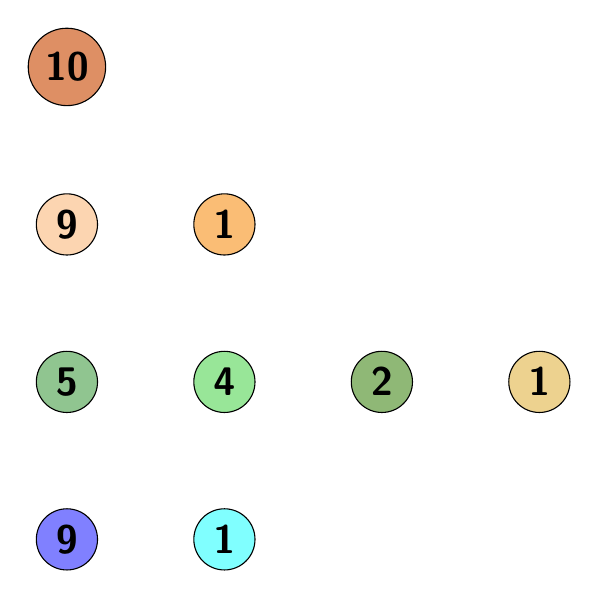
\begin{tikzpicture}[node distance=2cm, main node/.style={circle, draw, font=\sffamily\Large\bfseries}]

			\node[main node, fill=Bittersweet!50] (1) {10};
			\node[main node, fill=Apricot!50] (2) [below of=1] {9};
				\node[main node, fill=BurntOrange!50] (3) [right of=2] {1};
			\node[main node, fill=ForestGreen!50] (4) [below of=2] {5};
				\node[main node, fill=LimeGreen!50] (5) [right of=4] {4};
				\node[main node, fill=OliveGreen!50] (6) [right of=5] {2};
				\node[main node, fill=Goldenrod!50] (7) [right of=6] {1};
			\node[main node, fill=Blue!50] (8) [below of=4] {9};
				\node[main node, fill=Cyan!50] (9) [right of=8] {1};
			
			\tikzstyle{EdgeStyle}=[->, thick, blue]
			
			% main chain
			\Edge[](8)(4)
			\Edge[](4)(2)
			\Edge[](2)(1)
			
			% day 4 branches
			\Edge[](9)(5)
			
			% day 3 branches
			\Edge[](5)(2)
			\Edge[](6)(2)
			\Edge[](7)(3)
			
			% day 2 branches
			\Edge[](3)(1)
			
		\end{tikzpicture}
	\caption{Sample page-chain on day 4. Quorum size is $ M = 10 $, the numbers represent quorum participants with the same page. Despite malicious collusion and misbehaving nodes on day 3, most of day 4's quorum choose the correct chain with $ 10 + 9 + 1 + 5 + 4 + 2 = 31 $ total participants.}
	\label{fig:figure5}
\end{figure}

\subsection{Snapshot}

Similar to a page, a \textit{snapshot} is JSON-encoded textual database held by quorum nodes, but unlike pages, snapshots are short-term and volatile. They are used for propagating very new records and receiving records from other quorum nodes, and are only held and processed by quorum nodes in the current day. Snapshots contain three fields: \textit{originTime}, \textit{recentRecords}, and \textit{snapshotSig}, where \textit{originTime} is the timestamp when the snapshot was first created, \textit{recentRecords} is a list of DNS records, and \textit{snapshotSig} is the digital signature of \textit{originTime} and \textit{recentRecords}. When a hidden service operator informs a quorum node about a new record, the quorum node first confirms that the record is valid (described below) and if it is, it adds that record into \textit{recentRecords} and updates \textit{snapshotSig}. 

%todo: do I describe how records are validated?

Where $ snap_{x} $ is the current snapshot at propagation iteration $ x $, at each 15 minute mark each active quorum node $ node_{j} $ performs the following:

\begin{enumerate}
	\item Generates a new snapshot, labelled $ snap_{x+1} $, sets \textit{originTime} to the current time, creates \textit{snapshotSig}, and sets $ snap_{x+1} $ to be the currently active snapshot for collecting new records.
	\item Randomly selects $ M / 2 $ nodes from the $ M $ quorum nodes, defining \textit{swapSet}.
	\item With each node $ node_{k} $ in \textit{swapSet}, it swaps $ snap_{x} $ and \textit{pageSig} with node $ node_{k} $, receiving a snapshot $ s_{x, k} $ and signature $ sig_{x, k} $, and then verifies the validity of $ s_{x, k} $. For efficiency, if $ node_{k} $ in turn selects $ node_{j} $, no swap will need to take place.
	\item After all swapping is complete, $ node_{j} $
		\begin{enumerate}
			\item Archives $ snap_{x} $ and each $ s_{x, k} $ and $ sig_{x, k} $ for all $ k $ in \textit{swapSet}.
			\item Updates its copy of $ node_{k} $'s page by merging in $ s_{x-4, k} $, then confirming that $ sig_{x, k} $ verifies against the generated page. If not, it asks $ node_{k} $ for its page so that the discrepancy can be resolved.
			\item Updates its page by merging the contents of $ snap_{x-4} $ into \textit{recordList} and regenerates \textit{pageSig}.
			\item Deletes $ snap_{x-4} $.
			\item Increments $ x $.
		\end{enumerate}
\end{enumerate}


% Page identification? Is 4b right? Need to swap all known snapshots! Delete old snapshots!
\textit{TODO: this is incomplete. Quorum nodes send and receive a set of snapshots from other quorum nodes. They pass them along. After 4 rounds of share-with-50-percent the information should have reached all quorum nodes with a high probability, so the information can be safely added into the page and the signature updated. Likewise snapshots from other quorum nodes that are 4 rounds old can be added into its page, hence everyone will be in agreement, theoretically at least. Experiments needed and planned.}

\subsection{Synchronization}

Tor nodes must perform a full synchronization with the quorum nodes or node(s) mirroring the database before they are qualified to be picked as part of a quorum. Additionally, they may optionally synchronize in order to become a mirror of the database themselves.

Synchronization occurs in O(n) time, where $ n $ is the number of days since since first page was generated. This is possible because each quorum node contains the pages from all other quorum nodes, so the synchronizing node only has to ask a single node in the quorum for the pages contained by all other sister quorum nodes for each day. Once the node has queried the nodes all the way back to the first quorum it can then follow the selection procedure described above in the Page section.

\subsection{Registration Creation}

Any hidden service operator may claim any domain name that is not currently in use. As domain names cannot be purchased from a central authority, it is necessary to implement a system that introduces a cost of ownership. This performs three main purposes: 1) thwarts potential flooding of system with domain registrations, 2) introduces a cost of investment that improves the availability of hidden services, and 3) makes domain squatting more difficulty, where someone claims one or more domains on a whim for the sole purpose of denying them to others. As hidden service operators typically remain anonymous, it is difficulty for one to contact them and request relinquishing of a domain, nor is there a central authority to force relinquishing through a court order or other formal means. Therefore we introduce a proof-of-work scheme that makes registration computationally intensive but is also easily verified by anyone.

A domain registration consists of nine components: \textit{name}, \textit{subdomains}, \textit{contact}, \textit{timestamp}, \textit{consensusHash}, \textit{nonce}, \textit{pow}, \textit{recordSig}, and \textit{pubHSKey}. The variable \textit{central} consists of all fields except \textit{recordSig} and \textit{pow}.

\begin{description}
	\item[name] \hfill \\
		A required field that specifies the domain name that the hidden service operator wishes to obtain, up to 32 characters in length. Domain names uses the .tor TLD.
	\item[subdomains] \hfill \\
		Names of the subdomains used before \textit{name} and their destinations. For example {"sample", "a.b.tor"} generates sample.example.tor that resolves to a.b.tor. They can also point to .onion addresses or traditional Clearnet domain names. Each subdomain and their destinations may each be up to 32 characters in length, and up to 16 subdomains may be registered per registration. This is an optional field.
	\textit{contact} \hfill \\
		The fingerprint of the HS operator's PGP key, if he has one. If not or if he chooses to withhold this information, this field is left blank. If the fingerprint is listed, clients may query a public key server for this fingerprint, obtain the operator's PGP public key, and contact him over encrypted email.
	\textit{timestamp} \hfill \\
		The UNIX timestamp of when the operator created the registration and began the proof-of-work to validate it. This is a required field.
	\textit{consensusHash} \hfill \\
		The SHA-384 of the morning's consensus document at the time of registration, encoded in base64. This a provable and irrefutable timestamp, since it can be matched against archives of the consensus document. Quorum nodes will not accept registration records that reference a consensus document more than 48 hours old. This is also required.
	\textit{nonce} \hfill \\
		A required field consisting of four bytes that serve as a source of randomness for the proof-of-work, described below.
	\textit{pow} \hfill \\
		16 bytes that demonstrate the result of the proof-of-work. Encoded in base64 and required.
	\textit{recordSig} \hfill \\
		The digital signature of all preceding fields, signed using the hidden service's private key. Encoded in base64 and required.
	\textit{pubHSKey} \hfill \\
		A required field holding the base64-encoding of the hidden service's public key.
\end{description}

A record is made valid through the completion of the proof-of-work process. The hidden service operator must find a \textit{nonce} such that the SHA-384 of \textit{central}, \textit{pow}, and \textit{recordSig} is $ \leq 2^\textrm{difficulty} $, where \textit{difficulty} specifies the order of magnitude of the work that must be done. For each \textit{nonce}, \textit{pow} and \textit{recordSig} must be regenerated, which effectively forces the computation to be performed by a machine owned by the HS operator. While this scheme would not entirely prevent the operator from outsourcing the computation to a cloud service or to a secondary offline resource, the other machine would need the hidden service private key to regenerate \textit{recordSig}, which the operator can't reveal for obvious security reasons. However, the secondary resource could perform the scrypt computations in batch without generating \textit{recordSig}, but it would always perform more than the necessary amount of computation because it would could not take the SHA-384 hash and thus know when to stop. Furthermore, offloading the computation would still incur a cost to the hidden service operator, who would have to pay another party for the consumed computational resources. Thus the scheme always requires some cost when claiming a domain name. The valid and complete record is then represented in JSON format when transmitted and stored by quorum nodes.

\textit{TODO: specify how difficulty increases to counteract Moore's Law. Also, is the pow even necessary, or can that be regenerated by anyone?}

\subsection{Record Modification}

A hidden service operator may wish to update his registration with more current information. He can generate and broadcast a modification record, which contains updates to the field. The proof-of-work cost is a fourth of registration creation.

\subsection{Ownership Transfer}

Domain names may be transferred to a new owner from one hidden service operator to another. The transfer record contains the public key and signature of the originating owner and the public key of the new owner. The proof-of-work cost is an eighth of generating the domain name in the first place.

\subsection{Domain Renewal}

Domain names expire every 64 days, so they must be renewed periodically. To do this, a hidden service operator generates a renewal record and broadcasts it to the quorum nodes. The proof-of-work cost is a fourth of generating the domain name in the first place.

\subsection{Registration Deletion}

If a hidden service operator wishes to relinquish ownership rights over a domain name, they can issue a deletion record. This may happen if the hidden service key is compromised, the operator no longer has any use for the domain name, or for other reasons. The deletion record contains the hidden service public key and corresponding digital signature, and once issued to the quorum immediately triggers an expiration of that domain name, making it available to others by a creation record. There is no computational cost associated with a deletion record. 

\subsection{Broadcast}

A hidden service operator uses a Tor circuit to contact a quorum node. For security purposes, they must use the same entry node that their hidden service uses. Once the three-hop circuit has been established, they can use their exit node to give a record to the quorum node. That quorum node will add the record to their snapshot, which will be propagated to other quorum nodes and merged into pages for long-term storage.

\begin{figure}[htbp]
	\centering
	\begin{tikzpicture}[->, node distance=2.5cm, main node/.style={circle, fill=blue!20, draw, font=\sffamily\Large\bfseries}]

			\node[main node] (1) {$ Q_{1} $};
			\node[main node] (2) [right of=1] {$ Q_{1} $};
			\node[main node] (3) [right of=2] {};
			\node[main node] (4) [right of=3] {$ Q_{1} $};

			\node[main node] (5) [below of=1] {};
			\node[main node] (6) [right of=5] {$ Q_{1} $};
			\node[main node] (7) [right of=6] {};
			\node[main node] (8) [right of=7] {};
		  
			\node[main node, font=\small] (9) [below of=5] {$ N_{middle} $};
			\node[main node] (10) [right of=9] {};
			\node[main node, font=\small] (11) [right of=10] {$ N_{exit} $};
			\node[main node] (12) [right of=11] {$ Q_{1} $};

			\node[main node] (13) [below of=9] {};
			\node[main node] (14) [right of=13] {};
			\node[main node, font=\small] (15) [right of=14] {$ N_{entry} $};
			\node[main node] (16) [right of=15] {HS};
			
			% draw 1st and 2nd part of circuit
			\tikzstyle{EdgeStyle}=[bend right=12, -, green]
			\Edge[](16)(15)
			\Edge[](9)(15)
			
			% draw last part of circuit
			\tikzstyle{EdgeStyle}=[bend left=17, -, green]
			\Edge[](9)(11)
			
			% draw record moving from exit to 1st q. node
			\draw[thick, red, <-, postaction={decorate, decoration={text along path, text align=center, text={record}, raise=3pt}}] (6) to [bend left=20] (11){};
			
			% draw upper left propegation
			\tikzstyle{EdgeStyle}=[bend left=12, ->, blue]
			\Edge[](6)(2)
			\Edge[](2)(1)
			
			% draw upper right propegation
			\draw[thick, blue, postaction={decorate, decoration={text along path, text align=center, text={snapshot}, raise=3pt}}] (6) to [bend right=18] (4){};
			\draw[thick, blue, postaction={decorate, decoration={text along path, text align=center, text={snapshot}, raise=3pt}}] (4) to [bend left=25] (12){};

		\end{tikzpicture}
	\caption{HS operator broadcasts a record though a circuit (green) to a quorum node. The record propagates through snapshots.}
	\label{fig:figure5}
\end{figure}

\subsection{Registration Query}


binary hashtable, fallback alphabetized hashes of names/subdomains


When a Tor user wishes to visit example.tor, his client software must first perform a query to obtain the .onion address that corresponds to that domain name. The client must be able to verify that the received record originated from the desired hidden service, akin to SSL certificates on the Clearnet. Furthermore, the lookup must happen in an anonymous or privacy-enhanced manner and the details of the query must be handled behind-the-scenes, invisibly to the user. These policies satisfy our verifiability, privacy, and simplicity requirements.

At startup, the Tor client software may build a circuit to a quorum node or to any node mirroring the database. He then asks the node server for the domain name. Depending on the verification level specified by the client, this could be limited or large amounts of information. As we mentioned in the requirements section, it is impractical to require the client to download the entire DNS database to perform verification, so instead the client can perform various degrees of verification with minimal information.

At level 1, the server returns just returns the creation record. The client software then extracts the fields, uses \textit{pubHSKey} to confirm that \textit{recordSig} verifies the record, then confirms the proof-of-work. The client then uses \textit{pubHSKey} to generate the hidden service .onion address (eight bytes of the base32-encoded SHA-1 hash of the PKCS.1 DER encoding of \textit{pubHSKey}) and looks up the hidden service in the traditional manner. The lookup fails if the service has not published a recent hidden service desciptor to the distributed hash table, otherwise the lookup goes through. End-to-end verification is complete when \textit{pubHSKey} can be successfully used to encrypt the hidden service cookie and the service proves that it can decrypt $ sec $.

At level 2, the server return the record, the page that it was included in, the \textit{pageSig} from all quorum nodes on that day, and an archive of the consensus document. This is \textit{width verification}; the client can verify the authenticity of the consensus document, determine the old quorum members and their keys, hash the page, and then verify that all the \textit{pageSig}s verify against that hash. The client then proceeds with record verification and hidden service lookup, as specified in level 1.

At level 3, the server return the record, the page that contained that record, and the pages that form the chain below it. This is \textit{depth verification}; the client can confirm the length of the page-chain and records contained within. This is demanding both in computation and in bandwidth usage, but is an extremely thorough level of verification. 

\textit{TODO: at level 4, include consensus documents so that the old quorums can be found?}

At all levels, the server may return the introduction point for that hidden service, which the node can determine in advance by querying the distributed hash table and then cashing the result. This would significantly improve performance because the client can skip that step.


%At a high level, domain registrations are broadcasted through a Tor circuit to all committee nodes. Every node then analyses the registration as well as its knowledge of the chain and makes a decision. If the registration is invalid, the node rejects with an appropriate flag. If the domain name is already taken, the node returns a flag along with the pre-existing registration. Otherwise, it digitally signs its approval and the proposal itself and distributes this to the rest of the committee. It then waits for the rest of the committee votes. Since every Tor node has the up-to-date public keys of all other nodes due to the consensus documents, every committee member can verify the votes of all other committee members. Once the node confirms that all committee nodes received the same proposal and that a significant majority indicate that the domain is both valid and available, it adds the registration to its local storage. More importantly, the registration is recorded to an append-only endless scroll distributed within the Tor network. Thus domain names are consumed in a first-come-first-serve basis.

%The scroll is a distributed and highly redundant chained data structure that slowly rolls through the Tor network. The scroll is $ N $ by $ M $ in shape and consists of two primary components: \textit{blocks} and \textit{captures}. Blocks contain one or more captures, and blocks are duplicated across the $ M $ committee nodes. Each capture is a collection of information from one day; it contains the consensus document from the previous morning, a list of domain registrations approved that day, the approval sign-off digital signatures from the committee nodes on those registrations, the digital signatures from the committee indicating their approval of the integrity of the scroll, and the hash of the previous four captures. In this way, captures are fully verifiable and contain enough information to link to the previous capture, forming a chain. This chain is not held by any single Tor node, rather it is encapsulated within a rolling window of blocks $ N $ days deep. As the days progress, the captures in the oldest block are migrated to the current day's block, rolling the structure forward. Thus the scroll is divided across $ N $ blocks, with copies of each block held by $ M $ Tor nodes. I consider $ N = 16, M = 64 $ reasonable values, which would involve 1,024 nodes at any given time, although $ M $ can be easily changed even while the scroll is in use.

%This distributed system provides the ability to confirm a given domain name is not already in use, without relying on a single central authority. Assuming that the committee nodes are honest in their vote and trustworthy in their nature, this achieves all three properties of Zooko's Triangle. Even if the committee nodes are malicious, I believe I can introduce sufficient countermeasures to make it infeasible for an attacker to successfully manipulate the system, assuming that the majority of the Tor network is trustworthy. More research, design, and implementation is needed, but this I believe is a very promising approach.


% Each node then votes on the proposed registration. A vote consists of \textit{decision}, \textit{hash}, \textit{count}, \textit{root}, and \textit{signature} where \textit{decision} is either \textit{available}, \textit{unavailable}, or \textit{invalid}; \textit{hash} is the SHA256 of the registration it received; \textit{count} is the number of valid registrations it has in local storage; \textit{root} is the root node of the Merkle tree formed by those registrations; and \textit{signature} is the digital signature of the preceding fields.

% \textit{count} and \textit{root} will both be used to keep nodes synchronized with one another. Although I won't go into detail here, my plan calls for out-of-date nodes to attempt to synchronize with the node that advertises the highest \textit{count}. Synchronization also involves checking the votes, so falsely advertising a high \textit{count} isn't sufficient to mislead the network. \textit{root} is useful because it enables quick verification that nodes have synchronized lists and the use of a Merkle tree in general allows efficient synchronization when a node is out-of-date.

\section{Fault Tolerance}

Page wrapping stuff...